\documentclass[letterpaper,12pt,oneside]{book}
\usepackage[top=1in, left=1.25in, right=1.25in, bottom=1in]{geometry}
\usepackage{bachelorstitlepageUNAM}

\author{Luis Esteban Serrano Bermúdez}
\title{}
\faculty{Facultad de Ingeniería}
\degree{Ingeniero en Computación}
\supervisor{Dr. ... Tutor}
\cityandyear{Ciudad Universitaria, Cd. Mx., 2020}
\logouni{Escudo-UNAM}
\logofac{Escudo-FING}

\usepackage[T1]{fontenc}
\usepackage[utf8]{inputenc}
\usepackage[spanish,es-nodecimaldot,es-tabla]{babel}
\usepackage{graphicx}
\usepackage{subfigure}
\usepackage{tikz}

\graphicspath{{./figs/}}
\usepackage{setspace}

\begin{document}
	\frontmatter
	\maketitle
	\chapter*{}

	\begin{flushright}%
	  \emph{Dedicatoria ...}
	  \thispagestyle{empty}
	\end{flushright}

	\chapter{Agradecimientos}
	\spacing{1.5}

	\chapter{Resumen}

	\tableofcontents
	\listoffigures

	\chapter{Prólogo}
	    Este proyecto se ha desarrollado con la finalidad de añadir una mejora a los medidores de energía previamente realizados en el Instituto de Ingeniería de la UNAM. La finalidad de esta mejora es agregar una función de lectura de datos de registros del medidor de energía ADE7880 para poder analizar una gran cantidad de datos en poco tiempo.

	\mainmatter

%%%%%%%%%%%%%%%%%%%%%%%%%%%%%%%%%%%%%%%%%%%%%%%%%%%%%%%%%%%%%%%%%%%%%%%%%%%%%%%
%%%%%%%%%%%%%%%%%%%%%%%%%%%%%%%%% INTRODUCCIÓN %%%%%%%%%%%%%%%%%%%%%%%%%%%%%%%%
%%%%%%%%%%%%%%%%%%%%%%%%%%%%%%%%%%%%%%%%%%%%%%%%%%%%%%%%%%%%%%%%%%%%%%%%%%%%%%%
	\chapter{Introducción}
		
		\section{Computadora}
			Una computadora esta conformada por hardware y software. La parte de Hardware consta de 4 componentes: el procesador, que funciona como el cerebro; la unidad de entrada, por la cual los programas y los datos son ingresados; la unidad de salida por donde son presentados los los resultados y la memoria que es en donde se almacena el software y los datos.

			\subsection{Procesador}
				El procesador, tambien llamada como la Unidad Central de Procesamiento se puede clasificar en tres partes:
				
				\begin{itemize}
					\item \textbf{Registros}: Es una locación de almacenamiento dentro de la CPU en la cual se mantienem los datos y las direcciones de memoria durante la ejecución de una instrucción. Accesar a los registros de datos es más rápido que acceder a los datos en la memoria externa. Estos registros varían dependiendo del modelo del procesador.

					\item \textbf{Unidad Lógica Aritmética}: Es la calculadora numérica y evaluadora lógica de operaciones. Aquí se reciben los datos provenientes de la memoria principal o de los registros, realiza una operación lógica y si es necesario reescribe el resultado de vuelta al registro o memoria.

					\item \textbf{Unidad de Control}: Contiene las instrucciones lógicas del hardware, esta se encarga de decodificar y monitorear la ejecución de las instrucciones. Tambien funciona como árbitro de varios de los servicios del CPU, los cuiales se encuentran sincronizados por un reloj de sistema.
				\end{itemize}
	
		\section{Microprocesador}
			El procesador en una computadora, esta comprendido de varios circuitos integrados, mientras que un microprocesador es un procesador empaquetado en un único circuito integrado. Una microcomputadora usa un microprocesador como su CPU.

			Los microprocesadores vienen en diferentes presentaciones, 4-Bits, 8-Bits, 16-bits, 32-Bits e incluso en 64-Bits aunque estos últimos no son demasiado comunes como los anteriores. El número de bits corresponde al número de digitos binarios que el microprocesador puede manipular en las operaciones.

			El acceso de la memoria principal toma mucho más tiempo que el tiempo de reloj disponible por el CPU, por ello es que los microprocesadores de 32 y 64 Bits poseen una textit{memoria caché} de alta velocidad.

		\section{Medidor de Energía ADE7880}
			Este Circuito Integrado es un medidor de energía eléctrica trifasica de alta precisión, con interfaces de comunicación serial I$^2$C y SPI. Es adecuado para la medición de energía electrica activa, reactiva y aparente en varias configuraciones trifásicas, además posee registros de muestreo de formas de onda para todas las salidas del Convertidor Análogico Digital incluido en el Circuito Integrado.

			\subsection{Interfaces de Comunicación}
				El ADE7880 posee 3 puertos de comunicación serial SPI, I$^2$C Y HSDC, sin embargo por la configuración de los pines solo se pueden usar 2 tipos de configuraciones, una utilizando el puerto SPI únicamente y la segunda es usando los puertos I$^2$C Y HSDC.

				Se incluyen un conjunto de 3 registros que permiten verificar la comunicación con el CI\footnote{Circuito Integrado ADE7880 renombrado asi a partir de aqui para simplificar}. Los regsitros LAST\_OP (Address 0xEA01), LAST\_ADD (Address 0xE9FE) and LAST\_RWDATA se encargan de almacenar los datos, la dirección de registro y la naturaleza del acceso al registro (Lectura/Escritura) de la última comunicación exitosa respectivamente. El registro LAST\_RWDATA tiene 3 diferentes direcciones dependiendo de la longitud del registro de la última comunicación.

				\begin{table}[h]
					\begin{tabular}{ l | c }
						\textbf{Tipo de comunicación} & \textbf{Dirección de registro} \\
						\hline
						Lectura/ Escritura de 8-Bit & 0xE7FD \\
						Lectura/ Escritura de 16-Bit & 0xE9FF \\
						Lectura/ Escritura de 32-Bit & 0xE5FF \\
					\end{tabular}
					\caption{Direcciones de los registros de LAST\_RWDATA}
				\end{table}

				Después de cada comunicación exitosa los registros se actualizan con la información de la operación, 0xCA si fue escritura y 0x35 si es escritura y el dato que se leyó o escribió. Las operciones no completadas no se reflejan en estos registros asi como cuando se leen estos registros.

				\subsubsection{SPI (Serial Peripheral Interface)}
					El SPI de este CI siempre es esclavo en la comunicación y consiste en 4 pines de comunicación SCLK, MOSI, MISO Y SSA.
					El reloj para la transferencia de datos debe aplicarse al pin SCLK y todas las transferencias de datos se sincronizan con este reloj. El intercambio de información entrante en el CI se realiza en el pin MOSI en los flancos descendentes del reloj serial y el CI lo muestrea en los flancos ascendentes del reloj. Por el contrario la información saliente del CI se transfiere por el pin MISO en los flancos descendentes del reloj serial y el dispositivo maestro muestrea la información en los flancos ascendentes. El bit más significante de la palabra es intercambiado a la entrada. La másima frecuencia del reloj serial soportada por esta interfaz es de 2.5[MHz], el pin MISO se mantiene en alta impedancia mientras no hay intercambio de información.

					EL pin $\overline{SS}$ es utilizado para seleccionar entra más de un dispositivo si es que los hay. Para poder utilizar el dispositivo y realizar la comunicación entre ete y el dispositivo maestro este pin debe llevarse a un voltaje lógico bajo y permanecer así mientras dure la comunicación. Al cambiar el nivel lógico de este pin aborta la transferencia y para iniciar una nueva este se debe volver a poner a un voltaje lógico bajo.

				\subsubsection{I$^2$C (Inter Integrated Circuits)}
					Este CI posee una interfaz I$^2$C para la comunicación, implementada completamente como un hadware esclavo. El pin de intercambio de información SDA se encuentra localizado en el pin 38 y se encuentra compartido con el pin MOSI del puerto SPI, de igual manera el reloj serial SCL se encuentra compartido con el reloj serial del puerto SPI en el pin 36. La máxima frecuencia soportada por el reloj serial es de 400[kHz].

					La secuencia de transferencia del sistema I$^2$C consiste en el dispositivo maestro generando un condición de inicio para la transferencia cuando el bus se encuantra desocupado. El dispositivo maestro entonces transmite la direccion del dispositivo esclavo (0x70) y la dirección del regitro de la transferencia de datos en la transferencia de dirección inicial si el dispositivo esclavo reconoce entonces empieza la transferencia de datos. Esto continua hasta que el maestro emite una condición de parada y el bus queda de nuevo desocupado.

				\subsubsection{HSDC (High Speed Data Capture)}
					Debido a que para este proyecto es necesario el recopilar una gran cantidad de muestras a alta velocidad la documentación del Circuito Integrado ADE7880 recomienda, para la lectura de estos registros en específico, utilizar una interfaz propia de Analog Devices para este circuito llamada High Speed Data Capture (Captura de Datos a Alta Velocidad) por lo que es necesario configurar el microprocesador de manera que se pueda usar la comunicación I$^2$C como interfaz serial principal y la comunicación HSDC como secundaria usando el canal SPI del microcontrolador como esclavo, que recibirá toda la información de los registros de voltaje y corriente enviados por esta interfaz.

%%%%%%%%%%%%%%%%%%%%%%%%%%%%%%%%%%%%%%%%%%%%%%%%%%%%%%%%%%%%%%%%%%%%%%%%%%%%%%%
%%%%%%%%%%%%%%%%%%%%%%%%%%%%%%%%%%% FIRMWARE %%%%%%%%%%%%%%%%%%%%%%%%%%%%%%%%%%
%%%%%%%%%%%%%%%%%%%%%%%%%%%%%%%%%%%%%%%%%%%%%%%%%%%%%%%%%%%%%%%%%%%%%%%%%%%%%%%
	\section{Firmware}
		\subsection{Configuración del puerto I$^2$C}
			Este puerto se activa al encender el dispositivo o al realizar un reinicio de hardware, entonces el puerto I$^2$C queda seleccionado como interfaz de comunicación. Para evitar que al hacer cambios en el nivel de voltaje del pin $\overline{SS}$/HSA se cambie a la interfaz de comunicación SPI, se debe bloquear el puerto I$^2$C para ello se debe poner a 1 el Bit 1 (I2C\_LOCK) del registro CONFIG2, esto previene que al realizar cambios de voltaje en el pin $\overline{SS}$/HSA y el cambio a SPI no es posible hasta que se realize un reinicio de hardware o se reinicie todo el sistema.

			\begin{table}[h]
				\begin{tabular}{c | c | c}
					\textbf{Bit} & \textbf{Mnemonico} & \textbf{Valor predeterminado} \\
					\hline
					0 & EXTREFEN & 0 \\
					\hline
					1 & I2C\_LOCK & 1 \\
					\hline
					7:2 & Reservados & 0 \\
				\end{tabular}
				\caption{Valores del registro CONFIG2 que se deben transmitir para bloquear el puerto I$^2$C}
			\end{table}

			Este registro se accesa como si fuera un registro de 8-Bits por lo que los 6 Bits más significativos deben permanecer como 0. En este caso en particular se transmite 0x02 a la dirección de registro 0xEC01.

		\subsection{Configuración del puerto HSDC}
			Para configurar el puerto HSDC se debe escribir primero al registro HSDC\_CFG [0xE706] a traves del puerto I$^2$C la configuración con la que se van a estar enviando los datos a traves del puerto HSDC. Ya que se configura el puerto se habilita colocando el bit 6 (HSDCEN) en el registro CONFIG [0xE618] a 1, con esto se activa la comunicación.

			La configuracion que se ha decidido usar es tener el reloj a 8[MHz] con la transmision de registros en paquetes de 32-bits, no se agrega una brecha de 7 ciclos de reloj entre transmisiones y unicamente se transmitira el contenido de los registros de voltaje y corriente: IAWV, VAWV, IBWV, VBWV, ICWV, VCWV, e INWV, lo que permite que se realice la comunicación de manera más rápida. El pin de selccion de esclavo ($\overline{SS}$ ó Chip Select) se mantiene como activo en bajo. %AUN SE ESTA PROBNADO SI FUNCIONARIA CON ACYIVO E BAJO O SE DEBE USAR COMO ACTIVO EN ALTO


	\chapter{Resultados}
		Como se explicó al principio el desarrollo de este proyecto se pensó como una mejora a los medidores de energía anteriormente fabricados por el Instituto de Ingeniería por lo que este, solo se centró únicamente en la lectura de muestras a alta velocidad por parte del microcontrolador.

		\section{Lectura de Datos Usando el Canal SPI}
			En un principio el sistema medidor de energía estaba pensado para realizar la comunicación entre el microprocesador y el medidor ADE7880 con interfaz SPI sin embargo al momento de realizar las primeras pruebas, los registros correspondientes a los canales de medición de voltaje y corriente, pasado un tiempo los valores que se recuperan de los registros pierden coherencia lo que hace que los resultados sean inutiles para su análisis.

			Como se pueden ver en las graficas de voltaje (Graficas \ref{CanalVoltaje}) y corriente (Graficas \ref{CanalCorriente}) al usar el canal SPI para muestrear los registros de voltaje y corriente de los 3 canales estos entregaban valores que no reflejaban la energía que se suministraba y en algunos casos ni siquiera se actualizaban los valores que el dispositivo tiene inicialmente, ya que las pruebas que se hacían se realizaban con un simulador de voltaje y corriente controlado con lo cual era posible conocer el valor que se deseaba obtener.

			Después de realizar un par de pruebas más y obtener valores similares en todas las pruebas y siguiendo la recomendación que el manual del dispositivo para la lectura de esos registros se decidió cambiar el canal de comunicación de SPI por el HSDC con el cual se planea tener una lectura más rápida de los registros así como poder mantener la comunicación únicamente con los registros de voltaje y corriente de manera continua sin interaciones con los otros módulos del sistema de medición de energía.

			\begin{figure}[htbp]
				\subfigure[Canal de Voltaje A]{
					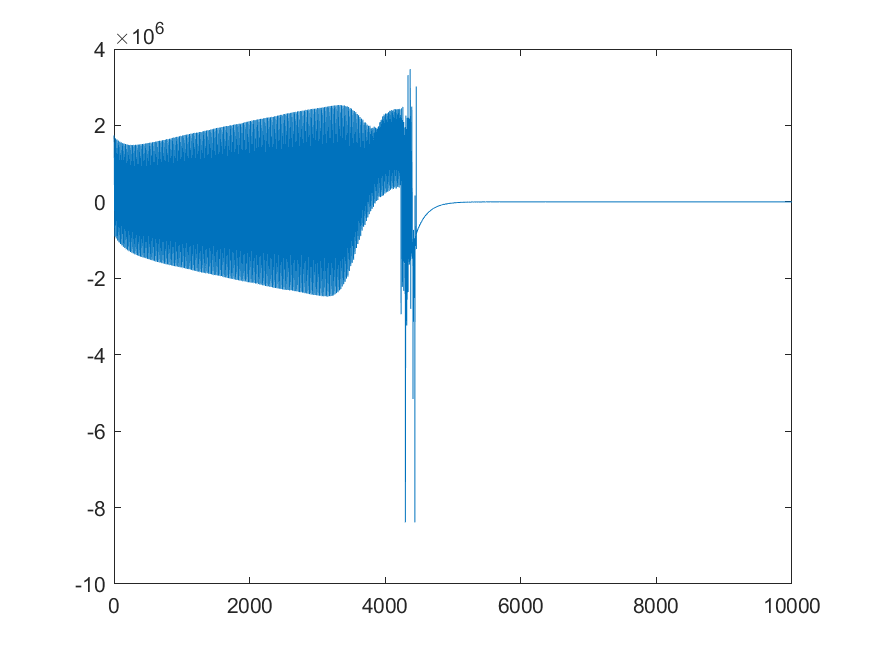
\includegraphics[scale = 0.6]{Pruebas de Muestreo/QS_140220.png}
				}
				\subfigure[Canal de Voltaje B]{
					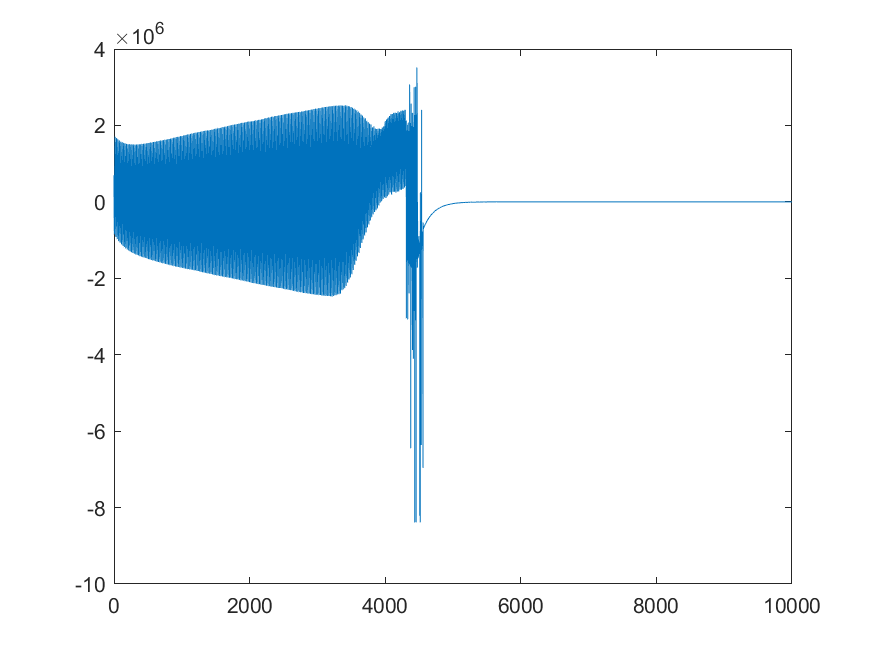
\includegraphics[scale = 0.6]{Pruebas de Muestreo/QS_140220-000000.png}
				}
				\subfigure[Canal de Voltaje C]{
					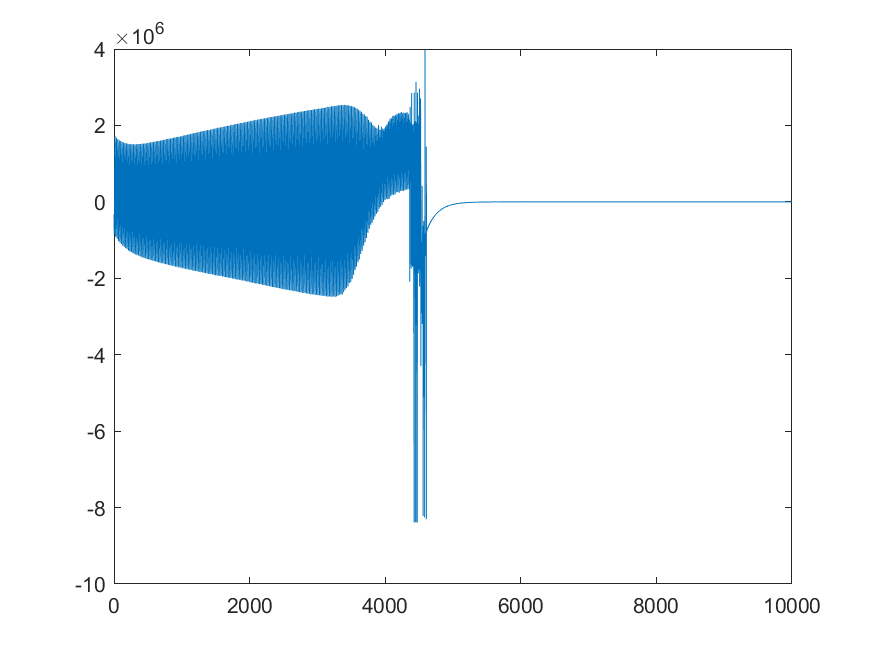
\includegraphics[scale = 0.6]{Pruebas de Muestreo/QS_140220-000001.png}
				}
				\caption[Gráficas de la primer prueba de los Canales de Voltaje]{Gráficas de la primer prueba de los Canales de Voltaje}
				\label{CanalVoltaje}
			\end{figure}

			\begin{figure}[htbp]
				\subfigure[Canal de Corriente A]{
					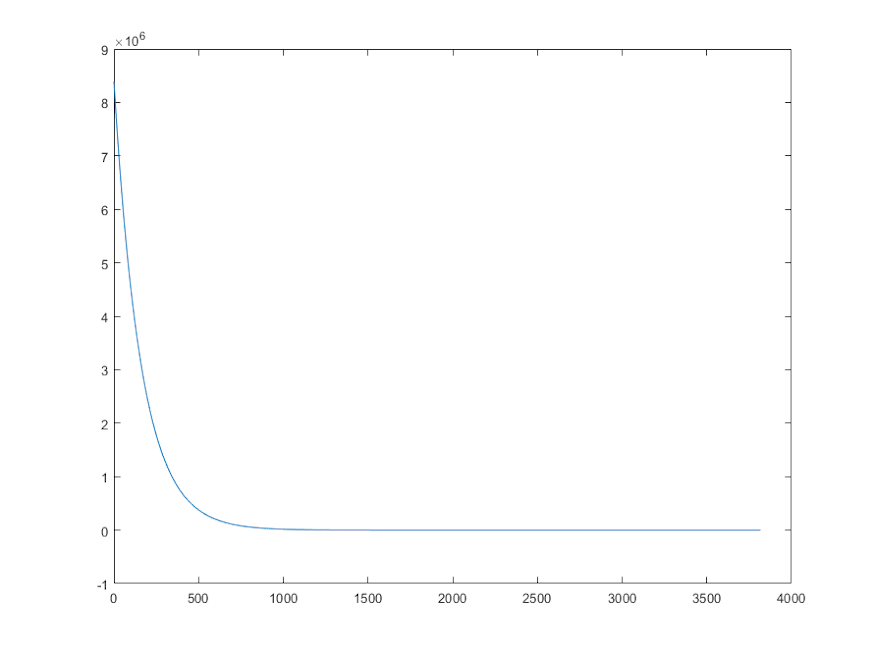
\includegraphics[width = 8.6cm, height = 6.7cm]{Pruebas de Muestreo/QS.png}
				}
				\subfigure[Canal de Corriente B]{
					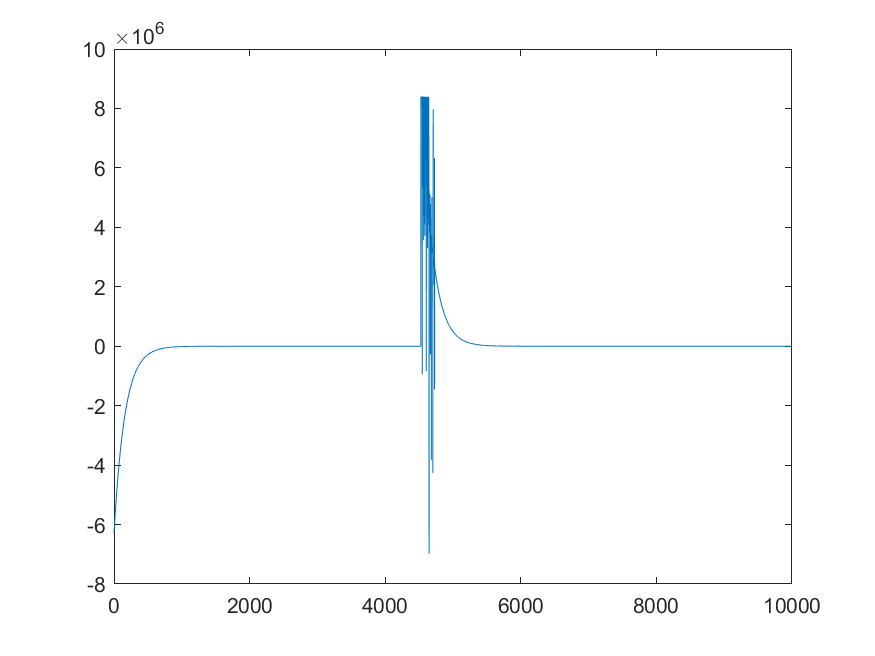
\includegraphics[scale = 0.6]{Pruebas de Muestreo/QS_140221.png}
				}
				\subfigure[Canal de Corriente C]{
					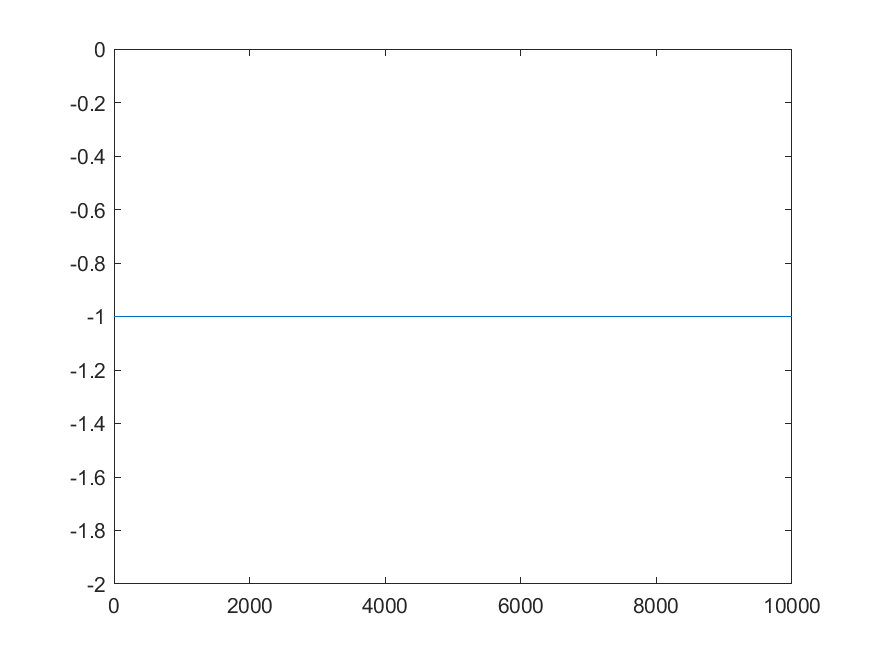
\includegraphics[scale = 0.6]{Pruebas de Muestreo/QS2.png}
				}
				\caption[Gráficas de la primer prueba de los Canales de Corriente]{Gráficas de la primer prueba de los Canales de Corriente}
				\label{CanalCorriente}
			\end{figure}

		%\section{Lectura de }

	\chapter{Conclusiones}

	%\bibliographystyle{humannat}
	%\bibliography{references}

	\backmatter%@sglvgdor
\end{document}